\documentclass[../../main.tex]{subfiles}
\begin{document}
\chapter{Intermediate Blocks, Motion Curves, and Using AZee Templates}
\label{ch:intermediate_blocks}

This chapter delves into the intricacies of generating intermediate blocks in multi-track representations discussed in chapter \ref{ch:multi-track} of Sign Language discourse, using a combination of procedural and artistic techniques. The approach discussed leverages the AZee model, which enables the representation of Sign Language discourses on a multi-track timeline, mapping directly to a non-linear editor. By employing motion templates and careful interpolation between keyframes, we aim to improve the naturalness and accuracy of synthesized Sign Language.


todo, chapter is structured as follows.. 

\section{Related Work}
\label{ch:intermediate_blocks:related_work}

\subsection{AZee Templates}
\label{ch:intermediate_blocks:related_work:azee_templates}

The AZee model offers a flexible and robust approach to representing sign language structures, especially proforms, by utilizing geometric templates that can be applied across various signing scenarios. For example, a rule such as place-prf(proform-vehicle, midssp) allows for the placement of a vehicle proform in the middle of the signing space(figure \ref{fig:azee_template_example}). This method leverages a consistent geometric system, enabling the natural synthesis of movements without relying on a fixed set of points, which is crucial for capturing the variability and dynamism inherent in sign language. This approach, as detailed underscores the system's ability to generate natural animations by focusing on higher-level linguistic structures rather than low-level positional data, thus improving the fluidity and realism of synthesized sign language animations \cite{filhol2018extending}.

TODO better way to put AZee templates

\begin{figure}
    \centering 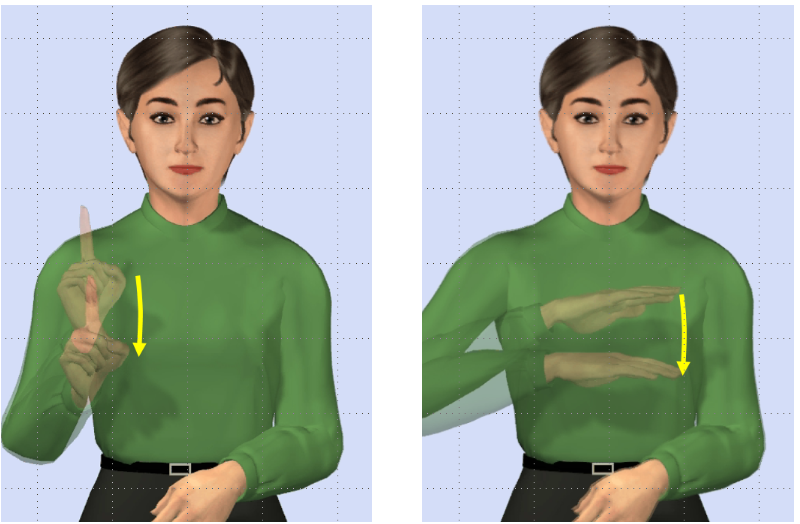
\includegraphics[width = 2.5in]{chapters/intermediate_blocks/images/azee_template_example.png}
    \caption{AZee Templates used by the Paula avatar}
    \label{fig:azee_template_example}
\end{figure}

Pre-animated animations are integrated into the AZee-Paula system through a hierarchical fallback mechanism that prioritizes naturalness by first attempting to match entire AZee expressions to pre-animated segments. If a perfect match is found, the system directly uses the pre-animated sequence, ensuring high-quality, fluid animations. When an exact match is not available, the system matches at a more granular level, utilizing templates that accommodate variations within the AZee expressions, such as different locations or motions. If template matching also fails, the system synthesizes the animation from lower-level constraints, ensuring flexibility while maintaining naturalness whenever possible.

In conclusion, the extensive work on motion curves, motion templates, and sign language animation provides essential groundwork for the techniques presented in this thesis. From the early applications of spacetime constraints to the integration of deep learning models, the evolution of these methods demonstrates the increasing sophistication in controlling and generating animations. Similarly, the use of templates and AZee models offers powerful frameworks for ensuring consistency and naturalness in sign language synthesis. These contributions collectively inform the intermediate block generation, motion curve stitching, and template reuse approaches that are central to this thesis, facilitating more fluid, adaptable, and realistic animations for Sign Language avatars.

\subsection{Motion Curves}
\label{ch:intermediate_blocks:related_work:motion_curves}

Motion curves, (often refered as function curves or F-curves), have been extensively used in 3D character animation to control the timing and spacing of movements. These curves provide a graphical representation of a parameter's change over time, making them an essential tool in achieving realistic and fluid motion in animations(figure \ref{fig:fcurves_blender}). Early foundational work by Witkin and Kass \cite{witkin1988spacetime} introduced spacetime constraints, which used optimization techniques to control motion curves in generating realistic animations under physical constraints. This idea has evolved, and modern techniques now integrate deep learning models with motion curves to enhance control and automate the generation of complex animations.

In the context of Sign Language, \cite{inproceedings} discuss the use of 3D motion analysis to accurately capture and animate sign language gestures by extracting motion curve parameters from sensors like Microsoft Kinect. These motion curves, which represent the trajectories of movements made during signing, are essential for animating virtual signers in a natural and precise manner. The paper highlights how these curves are mathematically defined, including their type, plane of motion, and velocity, which are then used to recreate realistic sign language animations, enhancing applications like sign language recognition and machine translation.

\begin{figure}
    \centering 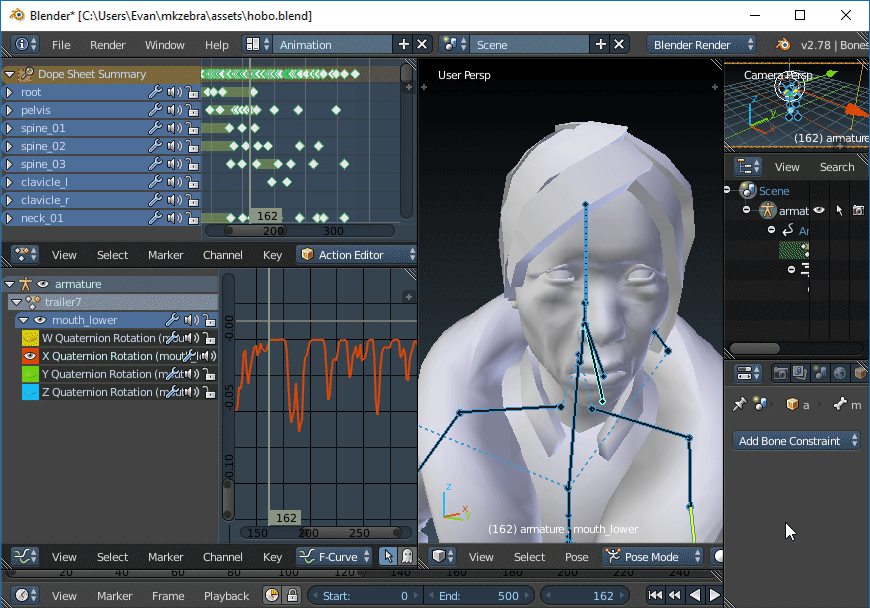
\includegraphics[width = 2.5in]{chapters/intermediate_blocks/images/fcurves_blender.png}
    \caption{F-curves in Blender}
    \label{fig:fcurves_blender}
\end{figure}

In recent research, deep learning methods have been employed to interpret and adapt F-curves for motion inbetweening tasks(figure \ref{fig:inbetweening_transformers}) \cite{10.1145/3550454.3555454}. However, traditional mathematical optimization techniques are still widely in use(figure \ref{fig:inbetweening_disney}) \cite{10.1145/3306346.3322938}.

\begin{figure}
    \centering 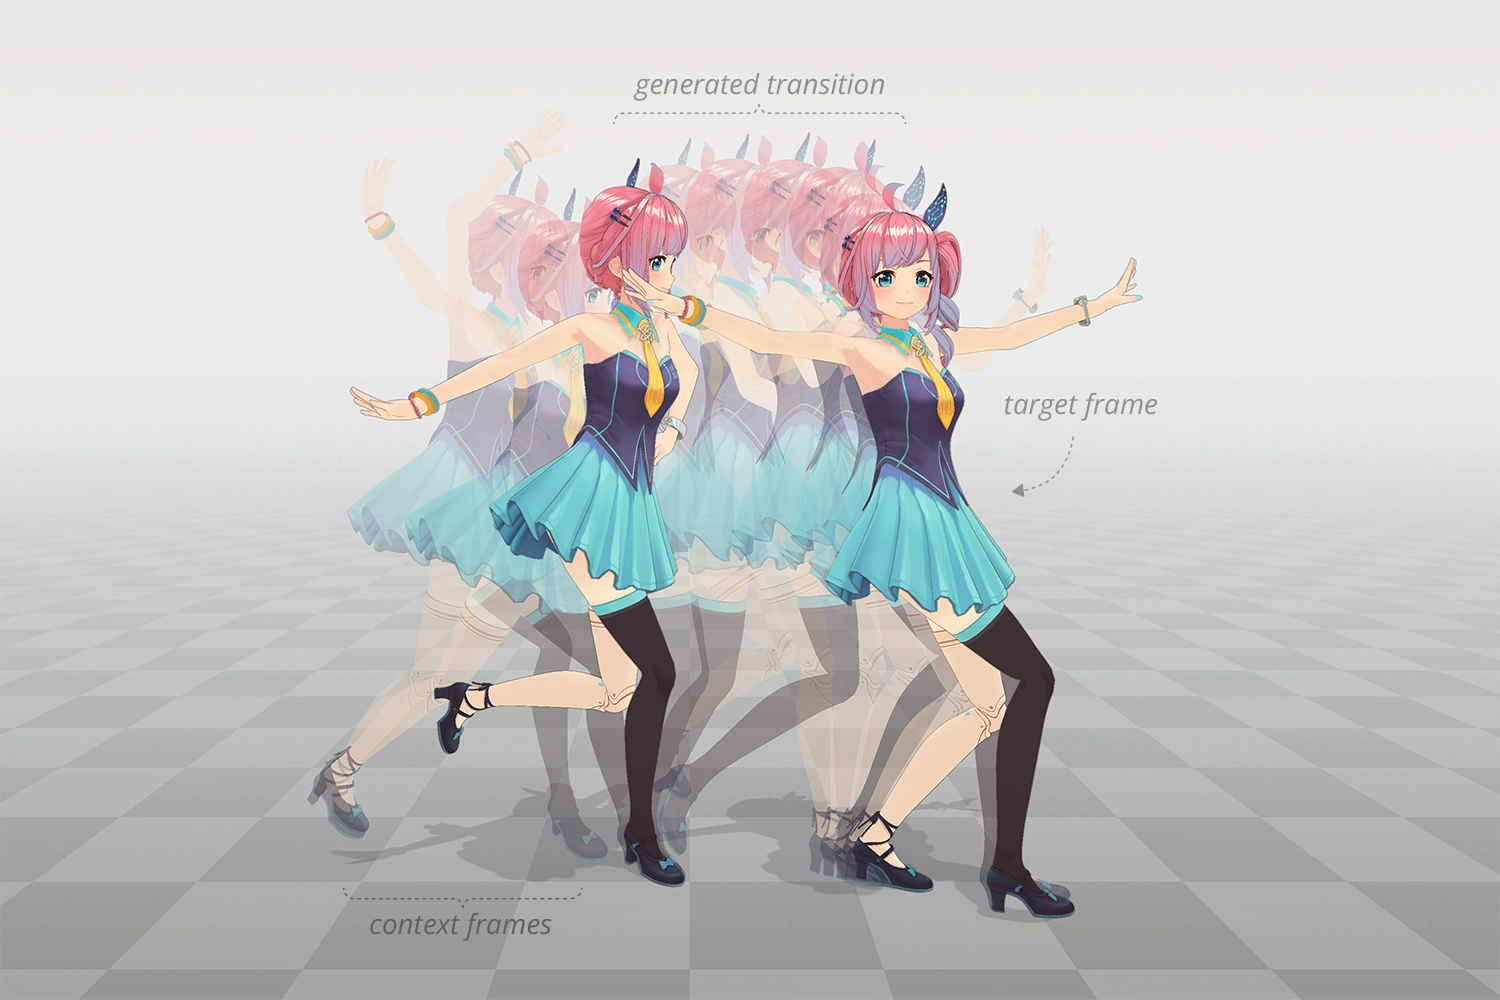
\includegraphics[width = 2.5in]{chapters/intermediate_blocks/images/inbetweening_transformers.png}
    \caption{Motion Inbetweening using 2 stage Transformers \cite{10.1145/3306346.3322938}}
    \label{fig:inbetweening_transformers}
\end{figure}

\begin{figure}
    \centering 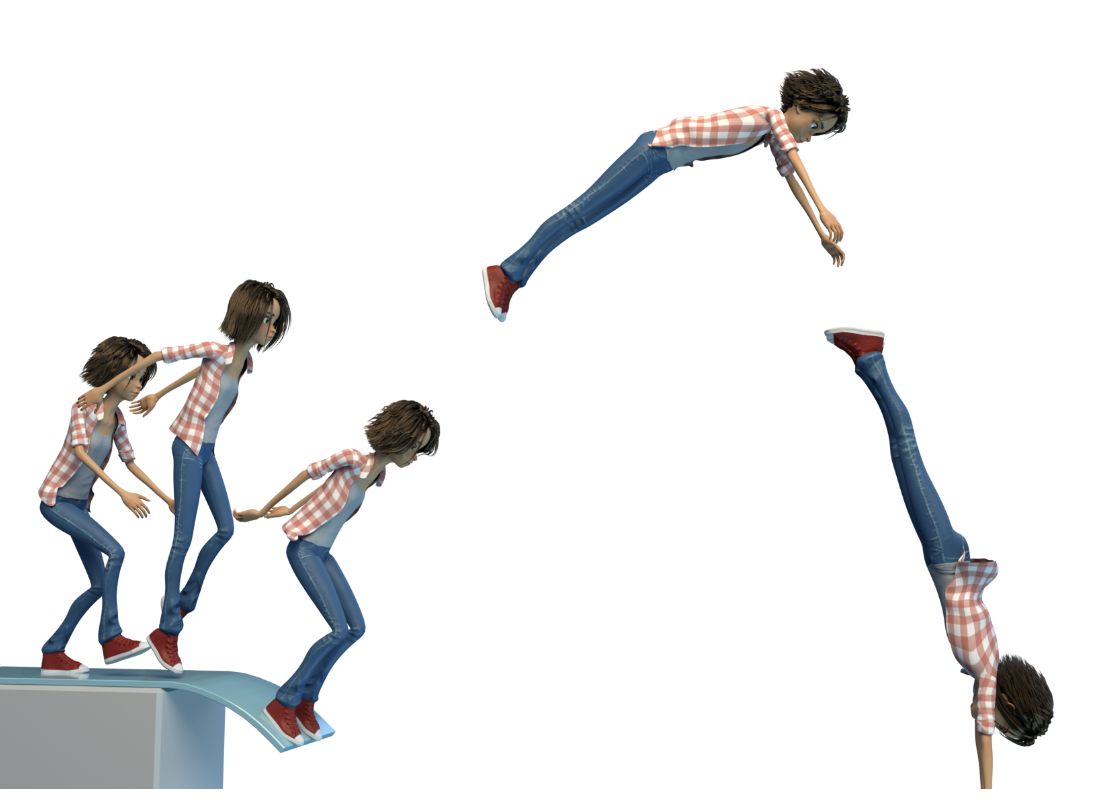
\includegraphics[width = 2.5in]{chapters/intermediate_blocks/images/inbetweening_disney.png}
    \caption{Rig Control using Tangent-Space Optimization}
    \label{fig:inbetweening_disney}
\end{figure}


\subsection{Motion Templates}
\label{ch:intermediate_blocks:related_work:motion_templates}

Motion templates offer a reusable framework for applying pre-defined motion patterns across different characters or scenarios. These templates are essentially built upon motion curves that define the motion's parameters, allowing for efficient replication and adaptation of complex motions. The concept of motion templates has been widely adopted in various fields, from character animation to robotic motion planning. Modern approaches often combine motion templates with machine learning techniques to facilitate the adaptation of these templates to new contexts, such as different character anatomies or environmental conditions.

In the context of character animation, motion templates can be particularly advantageous. The reusable nature of these templates allows for the consistent production of motion across different avatars while ensuring that the nuances of each motion are preserved. A method for controlling avatars using clustered motion segments from a large motion capture database was introduced by cite{10.1145/566654.566607}, enabling efficient real-time animation with intuitive user interfaces.

\section{Intermediate Block Generation}
\label{ch:intermediate_blocks:intermediate_block_generation}

Building on the concepts of motion curves and templates, intermediate block generation is a key process in creating smooth transitions between pre-animated and procedurally generated content. Interpolation techniques, such as linear and spline interpolation, are employed to generate intermediate poses or frames that maintain the semantic consistency of the intended sign.

The interpolation process discussed in this chapter utilizes a combination of linear and spline interpolation techniques, depending on the complexity of the motion being synthesized. Linear interpolation is straightforward and computationally efficient, making it suitable for simple transitions where the movement between keyframes is relatively uniform. However, for more complex motions—such as those involving intricate hand shapes or facial expressions—a spline-based approach is preferred. Splines allow for smoother transitions and better capture the nuances of human motion, which is essential for maintaining the naturalness of the synthesized Sign Language.

One of the key challenges in interpolation is ensuring that the intermediate poses remain semantically consistent with the intended sign. This is where the AZee model's multi-track approach proves advantageous. By representing each component of the sign (e.g., hand configuration, facial expression, body posture) as a separate track, the model allows for more precise control over the interpolation process. Each track can be interpolated independently, ensuring that the resulting poses are not only smooth but also semantically accurate.

In practice, the interpolation process is often iterative. Initial interpolations are generated and then evaluated for naturalness and consistency. If the resulting motion does not meet the desired criteria, adjustments are made—either by refining the interpolation technique or by tweaking the underlying keyframes. This iterative process continues until the synthesized motion achieves a level of quality that is acceptable for use in the final animation.

\section{Motion Curve Stitching}
\label{ch:intermediate_blocks:cruve_stitching}

Motion curve stitching refers to the process of combining different motion curves to create a continuous and seamless animation. In the context of Sign Language synthesis, this involves stitching together motion curves generated from pre-animated blocks, interpolated blocks, and procedural animations. The goal is to create a fluid and natural movement that accurately represents the intended sign.

The process of motion curve stitching begins with the identification of keyframes within each block. These keyframes represent critical points in the motion, such as the start and end of a sign or a change in hand configuration. Once these keyframes are identified, the corresponding motion curves are extracted and analyzed. The challenge here is to ensure that the motion curves from different blocks align correctly, both temporally and spatially. Misalignments can result in unnatural transitions or even incorrect signs, which would undermine the overall quality of the animation.

To address this challenge, the stitching process utilizes a combination of blending and warping techniques. Blending involves gradually transitioning from one motion curve to another, ensuring a smooth and continuous movement. Warping, on the other hand, involves adjusting the timing and spatial properties of the motion curves to ensure that they align correctly. These techniques are applied iteratively, with the resulting motion curves being evaluated for naturalness and accuracy.

The success of motion curve stitching depends heavily on the quality of the underlying motion curves. Poorly generated motion curves—whether due to inaccurate keyframes or inadequate interpolation—can lead to noticeable artifacts in the final animation. Therefore, it is essential to ensure that each step of the motion synthesis process, from keyframe selection to interpolation, is performed with a high degree of precision.

\section{Reusing Motion Templates}
\label{ch:intermediate_blocks:reusing_motion_templates}

Motion templates are pre-defined motion patterns that guide the synthesis of new animations. In the context of Sign Language synthesis, these templates serve as a blueprint for generating intermediate blocks and stitching together motion curves. The use of motion templates allows for greater consistency and control over the final animation, as the templates encode expert knowledge about how certain signs should be performed.

The creation of motion templates is a complex process that involves both empirical observation and artistic input. Typically, templates are derived from motion capture data, which provides a detailed record of how native signers perform specific signs. This data is then analyzed to identify common patterns and features, such as the timing of hand movements or the relationship between facial expressions and hand configurations. These patterns are encoded into the motion templates, which can then be applied to new signs or sequences.

One of the key advantages of using motion templates is that they allow for greater flexibility in the synthesis process. By applying different templates to the same set of keyframes, it is possible to generate multiple variations of the same sign, each with its own unique characteristics. This flexibility is particularly useful in the context of Sign Language synthesis, where the meaning of a sign can vary depending on factors such as context or the emotional state of the signer.

The use of motion templates also facilitates the process of motion curve stitching. By providing a consistent framework for generating motion curves, the templates help ensure that the resulting curves align correctly and produce a natural and seamless animation. In practice, this means that the stitching process is less reliant on manual adjustments and can be performed more efficiently.

However, the use of motion templates is not without its challenges. One of the main issues is the potential for overfitting, where the templates are too closely tailored to the specific motions they were derived from and do not generalize well to new signs or contexts. To mitigate this risk, it is important to ensure that the templates are sufficiently flexible and can be adapted to a wide range of motions.

\section{Results}
\label{ch:intermediate_blocks:results}

The application of the techniques discussed in this chapter has yielded promising results in the synthesis of realistic Sign Language avatars. The use of intermediate blocks and motion curve stitching has significantly improved the naturalness and accuracy of the animations, particularly in cases where complex motions or transitions are required. The incorporation of motion templates has also contributed to greater consistency and control over the final animations, allowing for more precise and contextually appropriate representations of Sign Language.

One of the key metrics used to evaluate the success of the synthesis process is the naturalness of the resulting animations. This is typically assessed through a combination of qualitative and quantitative measures, such as user studies and motion analysis. In user studies, participants are asked to rate the naturalness of the animations, as well as their comprehensibility and emotional expressiveness. The results of these studies have generally been positive, with participants reporting high levels of satisfaction with the synthesized animations.

Quantitative measures, such as the analysis of motion trajectories and timing, have also shown improvements in the quality of the synthesized animations. The use of motion templates, in particular, has led to more consistent and accurate motion curves, reducing the need for manual adjustments and increasing the overall efficiency of the synthesis process.

However, there are still areas where further improvements are needed. For example, while the current system performs well for common signs and phrases, it can struggle with more complex or less frequently used signs. Additionally, the system's reliance on pre-animated blocks and motion capture data means that it may not always be able to generate novel motions or adapt to new contexts. These limitations highlight the need for continued research and development in this area.

\section{Discussion}
\label{ch:intermediate_blocks:discussion}

The techniques discussed in this chapter represent a significant step forward in the synthesis of realistic Sign Language avatars. By combining procedural and artistic techniques, and by leveraging the AZee model and motion templates, it is possible to generate animations that are both natural and accurate. However, there are still challenges to be addressed, particularly in terms of scalability and generalization.

One of the main challenges is the need for large amounts of motion capture data to create high-quality motion templates. While motion capture provides a detailed and accurate record of how signs are performed, it is also time-consuming and expensive to collect. This limits the scalability of the current approach and may make it difficult to extend the system to cover the full range of signs used in different Sign Languages.

Another challenge is the need for greater flexibility in the synthesis process. While the use of motion templates provides a consistent framework for generating animations, it can also be somewhat rigid, making it difficult to adapt to new signs or contexts. Future work in this area could focus on developing more flexible and adaptive templates, as well as exploring new methods for generating novel motions.

Finally, there is the issue of generalization. The current system performs well for common signs and phrases, but it may not always be able to generate accurate representations of more complex or less frequently used signs. This highlights the need for further research into how the system can be improved to better handle the full range of signs used in different Sign Languages.

Despite these challenges, the results achieved so far are encouraging, and there is considerable potential for further improvements in the future. By continuing to refine and develop the techniques discussed in this chapter, it may be possible to create a system that can generate realistic and accurate Sign Language animations for a wide range of applications.

\end{document}